\fancyhead[L]{\small\textsf{\textbf{MỤC 1.1}\quad Bốn cách biểu diễn một hàm số}}
\fancyhead[R]{\small\textsf{\textbf{19}}}

\begin{multicols}{2}
\fontsize{8.5pt}{10.8pt}\selectfont
\setlength{\abovedisplayskip}{2pt}
\setlength{\belowdisplayskip}{2pt}

\begin{enumerate}
\item[(b)] Khi nào mức tiêu thụ điện năng đạt thấp nhất? Khi nào đạt cao nhất? Các thời điểm này có vẻ hợp lý không?
\end{enumerate}

\begin{center}
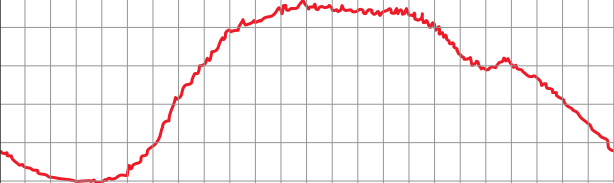
\includegraphics[width=0.88\linewidth]{images/p0054_graph_1.png}
\end{center}

\vspace{0.2cm}
\noindent
\textbf{24.} Ba vận động viên cùng tranh tài trong một cuộc chạy đua cự ly 100 mét. Đồ thị dưới đây mô tả quãng đường chạy được như một hàm số theo thời gian của mỗi vận động viên. Hãy diễn đạt bằng lời những gì đồ thị cho biết về cuộc đua này. Ai là người chiến thắng cuộc đua? Có phải tất cả các vận động viên đều hoàn thành cuộc đua không?

\begin{center}
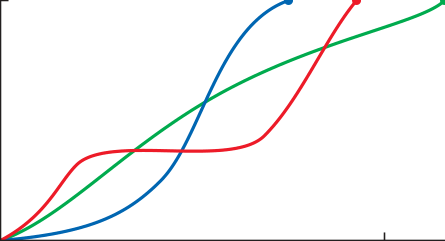
\includegraphics[width=0.88\linewidth]{images/p0054_graph_2.png}
\end{center}

\noindent
\textbf{25.} Hãy phác thảo một đồ thị ước chừng của nhiệt độ ngoài trời như một hàm số theo thời gian trong một ngày mùa xuân điển hình.

\vspace{0.15cm}
\noindent
\textbf{26.} Hãy phác thảo một đồ thị ước chừng về số giờ có ánh sáng ban ngày như một hàm số theo thời gian trong năm.

\vspace{0.15cm}
\noindent
\textbf{27.} Hãy phác thảo một đồ thị ước chừng về lượng cà phê của một nhãn hiệu cụ thể bán được tại một cửa hàng như một hàm số theo giá của loại cà phê đó.

\vspace{0.15cm}
\noindent
\textbf{28.} Hãy phác thảo một đồ thị ước chừng về giá trị thị trường của một chiếc xe ô tô mới như một hàm số theo thời gian trong khoảng thời gian 20 năm. Giả sử chiếc xe được bảo dưỡng tốt.

\vspace{0.15cm}
\noindent
\textbf{29.} Một chủ nhà cắt cỏ vào mỗi buổi chiều thứ Tư hàng tuần. Hãy phác thảo một đồ thị ước chừng về chiều cao của cỏ như một hàm số theo thời gian trong suốt khoảng thời gian bốn tuần.

\vspace{0.15cm}
\noindent
\textbf{30.} Một chiếc máy bay cất cánh từ một sân bay và hạ cánh sau đó một giờ tại một sân bay khác cách 400 dặm. Nếu $t$ biểu thị thời gian tính bằng phút kể từ khi máy bay rời nhà ga, gọi $x(t)$ là khoảng cách theo phương ngang đã bay và $y(t)$ là độ cao của máy bay.
\begin{enumerate}[label=(\alph*), itemsep=1pt, topsep=2pt, leftmargin=*]
\item Phác thảo một đồ thị khả dĩ của $x(t)$.
\item Phác thảo một đồ thị khả dĩ của $y(t)$.
\item Phác thảo một đồ thị khả dĩ của tốc độ mặt đất.
\item Phác thảo một đồ thị khả dĩ của vận tốc theo phương thẳng đứng.
\end{enumerate}

\columnbreak

\noindent
\textbf{31.} Các số đo nhiệt độ $T$ (tính theo $^\circ\text{F}$) được ghi lại hai giờ một lần từ nửa đêm đến 2:00 chiều tại Atlanta vào một ngày trong tháng Sáu. Thời gian $t$ được đo bằng giờ tính từ nửa đêm.

\begin{center}
\setlength{\tabcolsep}{3.5pt}
\begin{tabular}{|c|c|c|c|c|c|c|c|c|}
\hline
$t$ & 0 & 2 & 4 & 6 & 8 & 10 & 12 & 14 \\ \hline
$T$ & 74 & 69 & 68 & 66 & 70 & 78 & 82 & 86 \\ \hline
\end{tabular}
\end{center}

\begin{enumerate}[label=(\alph*), itemsep=1pt, topsep=2pt, leftmargin=*]
\item Sử dụng các số liệu để phác thảo một đồ thị ước chừng của $T$ như một hàm số theo $t$.
\item Sử dụng đồ thị của bạn để ước lượng nhiệt độ vào lúc 9:00 sáng.
\end{enumerate}

\vspace{0.15cm}
\noindent
\textbf{32.} Các nhà nghiên cứu đã đo nồng độ cồn trong máu (BAC) của tám đối tượng nam trưởng thành sau khi uống nhanh 30 mL ethanol (tương đương với hai đơn vị đồ uống có cồn tiêu chuẩn). Bảng bên dưới thể hiện dữ liệu thu được bằng cách tính trung bình BAC (đơn vị g/dL) của tám người này.
\begin{enumerate}[label=(\alph*), itemsep=1pt, topsep=2pt, leftmargin=*]
\item Sử dụng các số liệu để phác thảo đồ thị của BAC như một hàm số theo $t$.
\item Sử dụng đồ thị của bạn để mô tả tác động của cồn thay đổi như thế nào theo thời gian.
\end{enumerate}

\begin{center}
\setlength{\tabcolsep}{5pt}
\begin{tabular}{|c|c||c|c|}
\hline
\rowcolor{stewartcyan!15} $t$ (giờ) & BAC & $t$ (giờ) & BAC \\ \hline
0 & 0 & 1.75 & 0.022 \\
0.2 & 0.025 & 2.0 & 0.018 \\
0.5 & 0.041 & 2.25 & 0.015 \\
0.75 & 0.040 & 2.5 & 0.012 \\
1.0 & 0.033 & 3.0 & 0.007 \\
1.25 & 0.029 & 3.5 & 0.003 \\
1.5 & 0.024 & 4.0 & 0.001 \\ \hline
\end{tabular}
\end{center}
\vspace{-0.1cm}
{\scriptsize \textit{Nguồn:} Phỏng theo P. Wilkinson và các cộng sự, ``Pharmacokinetics of Ethanol after Oral Administration in the Fasting State,'' \textit{Journal of Pharmacokinetics and Biopharmaceutics} 5 (1977): 207--24.}

\vspace{0.25cm}
\noindent
\textbf{33.} Nếu $f(x) = 3x^2 - x + 2$, hãy tìm $f(2)$, $f(-2)$, $f(a)$, $f(-a)$, $f(a + 1)$, $2f(a)$, $f(2a)$, $f(a^2)$, $[f(a)]^2$, và $f(a + h)$.

\vspace{0.2cm}
\noindent
\textbf{34.} Nếu $g(x) = \dfrac{x}{\sqrt{x + 1}}$, hãy tìm $g(0)$, $g(3)$, $5g(a)$, $\frac{1}{2}g(4a)$, $g(a^2)$, $[g(a)]^2$, $g(a + h)$, và $g(x - a)$.

\vspace{0.3cm}
\noindent
{\color{stewartcyan}\textbf{35--38}}\quad Tính tỉ số gia (tỉ sai phân) cho hàm số đã cho. Hãy rút gọn câu trả lời của bạn.

\vspace{0.15cm}
\noindent
\textbf{35.} $f(x) = 4 + 3x - x^2, \qquad \dfrac{f(3 + h) - f(3)}{h}$

\vspace{0.15cm}
\noindent
\textbf{36.} $f(x) = x^3, \qquad \dfrac{f(a + h) - f(a)}{h}$

\vspace{0.15cm}
\noindent
\textbf{37.} $f(x) = \dfrac{1}{x}, \qquad \dfrac{f(x) - f(a)}{x - a}$

\vspace{0.15cm}
\noindent
\textbf{38.} $f(x) = \sqrt{x + 2}, \qquad \dfrac{f(x) - f(1)}{x - 1}$

\vspace{0.2cm}
\noindent
{\color{stewartcyan}\rule{\linewidth}{1.2pt}}

\end{multicols}